\documentclass[]{article}
\usepackage{graphicx}
\usepackage{float}
\usepackage{amsmath}
%\usepackage[]{hyperref}
% Title Page
\title{Lab 2}
\author{
	Alex Taglieri
	\\
	Andrew Kacherski
	}

\begin{document}
\maketitle
\newpage
\
\raggedright


\pagenumbering{arabic}
\section{Introduction and Background}

This lab explores the effects of springs in series and in parallel, and shows the how position, velocity, and acceleration are related for mass-spring systems in simple harmonic motion.

The position of an object in simple harmonic motion is described by the following equation:

\begin{equation}\label{position}
x(t)=Acos(\omega t + \phi)
\end{equation}

In this equation, \textit{A} represents the wave's amplitude, \textit{ $\omega $} is the angular frequency (in $ \frac{rad}{sec}$), \textit{t} is time (measured in seconds), and \textit{$ \phi $} is the phase angle, which is used to offset the wave in the horizontal direction and can often be taken as 0.

The object's velocity follows Expression \ref{velocity}. Notice that it's the derivative of Equation \ref{position}:

\begin{equation}\label{velocity}
v(t)=-A\omega sin(\omega t + \phi)
\end{equation}

Finally, the object's acceleration behaves according to Equation \ref{acceleration}, which is once again the derivative of Velocity (Equation \ref{velocity}).

\begin{equation}\label{acceleration}
a(t)=-A\omega^2 cos(\omega t + \phi)
\end{equation}

The force exerted on an object by a spring that's been stretched is given by Hooke's law:

\begin{equation}\label{fkx}
f=kx
\end{equation}

Here, \textit{f} represents the force, \textit{k} is the spring constant (which will be explored in the most detail in this lab), and \textit{x} is the displacement.

When two springs are in series, the resultant k-value (which determines the force, as Equation \ref{fkx} suggests) follows the Equation for Springs in Series:

\begin{equation}\label{seriesSpring}
k_{series}=\frac{1}{\frac{1}{k_1} + \frac{1}{k_2}}
\end{equation}

Note that if \textit{$k_1$} and \textit{$ k_2 $} are the same then the resultant \textit{k} value becomes $ \frac{k}{2} $.

For springs in parallel, the resultant \textit{k} value is given by Equation \ref{parallelSpring}:

\begin{equation}\label{parallelSpring}
k_{parallel} = k_1 + k_2
\end{equation}

Once again, if \textit{$k_1$} and \textit{$ k_2 $} are the same then the resultant \textit{k} value is $ 2k $.

Putting these two equations together, when four springs are arranged such that two are in series and two are in parallel, if all four springs have similar \textit{k}-values then the resultant \textit{k}-value is just \textit{k}. The derivation is shown in Equation \ref{parallelInSeries}.

\begin{equation}\label{parallelInSeries}
k_{seriesParallel}=\frac{1}{\frac{1}{k_1+k_2} + \frac{1}{k_3+k_4}}
\end{equation}

Assume $k_1 = k_2 = k_3 = k_4$:

\begin{equation}\label{parallelInSeries2}
\begin{split}
k_{series}&=\frac{1}{\frac{1}{k+k} + \frac{1}{k+k}} \\
&=\frac{1}{\frac{1}{2k} + \frac{1}{2k}} \\
&=\frac{1}{\frac{2}{2k}}\\
&=\frac{1}{\frac{1}{k}}\\
&=k
\end{split}
\end{equation}



\section{Procedure}

The general strategy is to measure the \textit{k}-value of just one spring, then measure the \textit{k}-value of 4 springs in parallel and series, and then set both systems in oscillation and compare them.

Hang the mass hanger from just one spring. Put 50 grams on the hanger and then zero the scale. Then start the mass at 200 grams and increase the mass by 200 grams at a time until the mass is 1000 grams, recording the displacement for each step. Calculate the k-value. 
Repeat the procedure for the 4-spring arrangement, with the springs both in parallel and in series.

Then set the system in motion with 600 grams of mass for the 4-spring arrangement and record the position over time. Finally, set the 1-spring arrangement in motion with 300 grams of mass hanging.


\section{Results}

The single spring we tested had a \textit{k}-value of 33.21. The masses were within \textit{0.5g} of their expected mass.

The 4-spring combination had a resultant k-value of 32.82. This is within 1 \textit{$\frac{N}{m}$} of the expected value - an error of about 3\%.

The angular frequency observed for one spring was 10.45, and the angular frequency for all four springs was 7.43. Since the \textit{k}-value was the same, the discrepancy can be explained because there was a different mass on the system.

\begin{figure}[H]
	\centering
	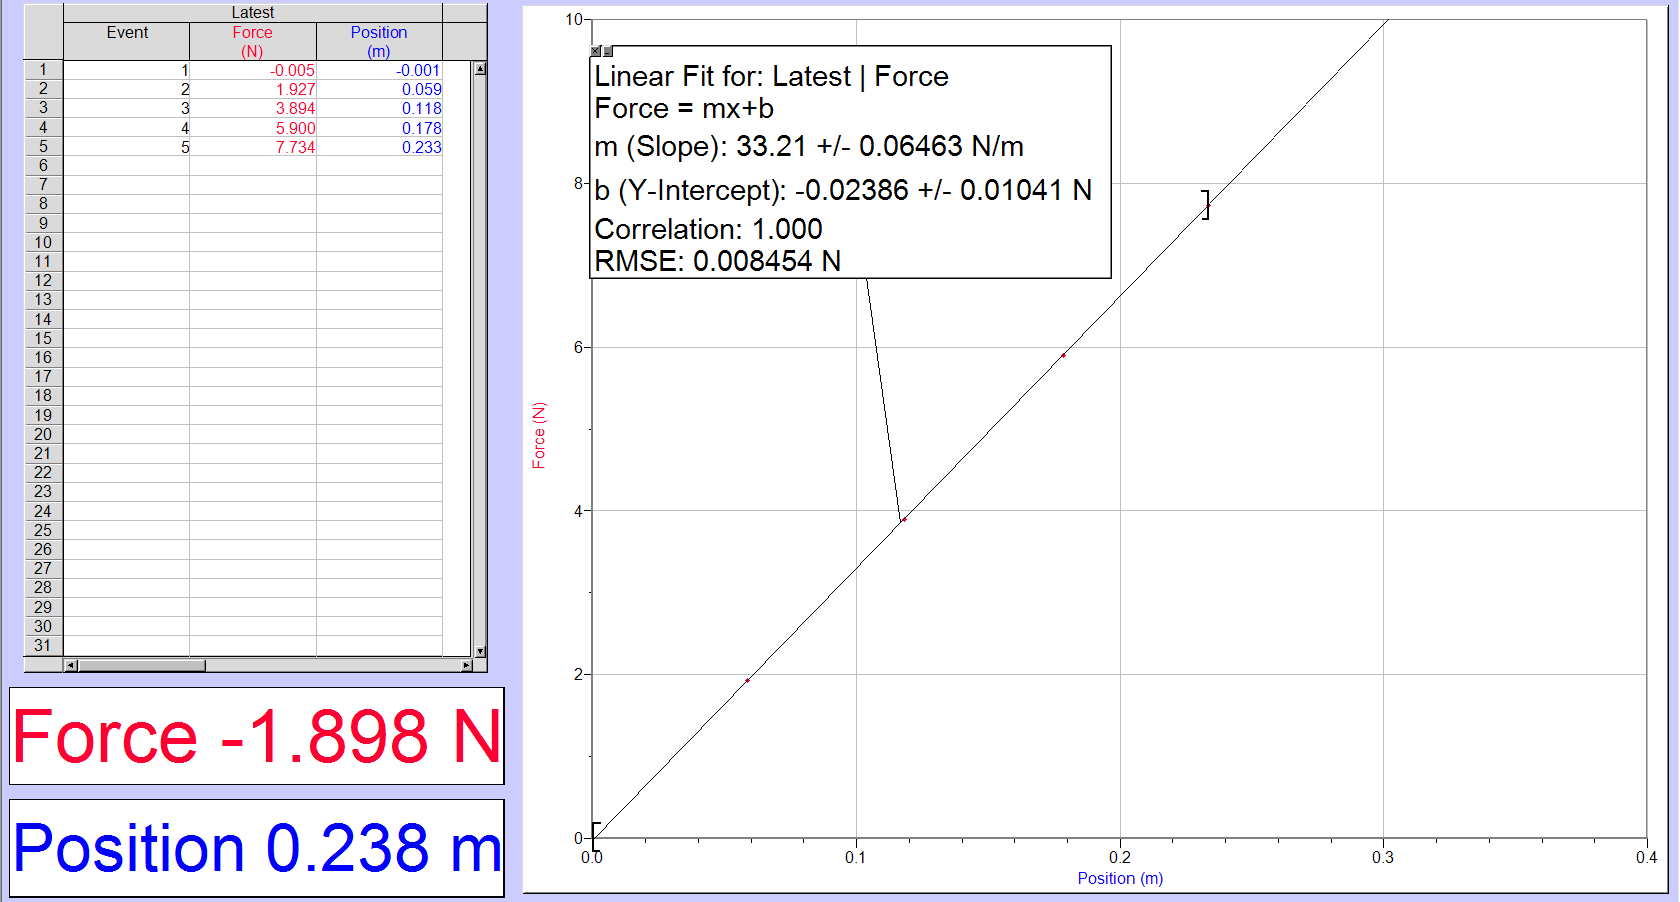
\includegraphics[width=\textwidth]{res/1_1_spring}
	\caption{Oscillations of Both Springs}
	\label{fig:Oscillations of Both Springs}
\end{figure}

\begin{figure}[H]
	\centering
	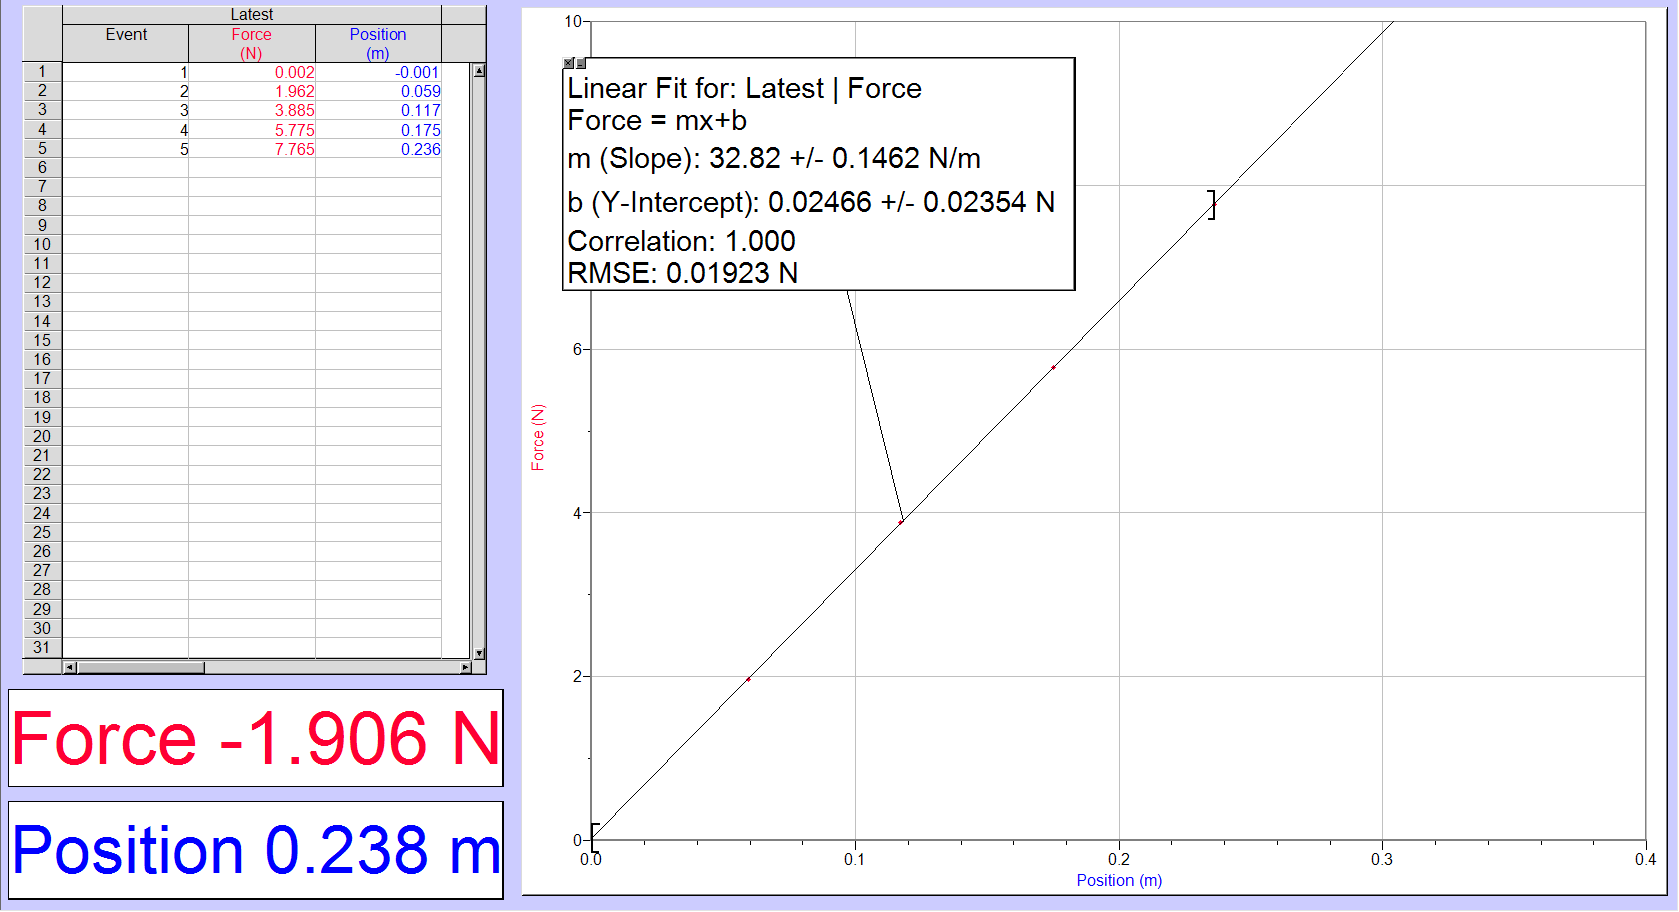
\includegraphics[width=\textwidth]{res/1_4_spring}
	\caption{Oscillations of Both Springs}
	\label{fig:Oscillations of Both Springs}
\end{figure}

\begin{figure}[H]
	\centering
	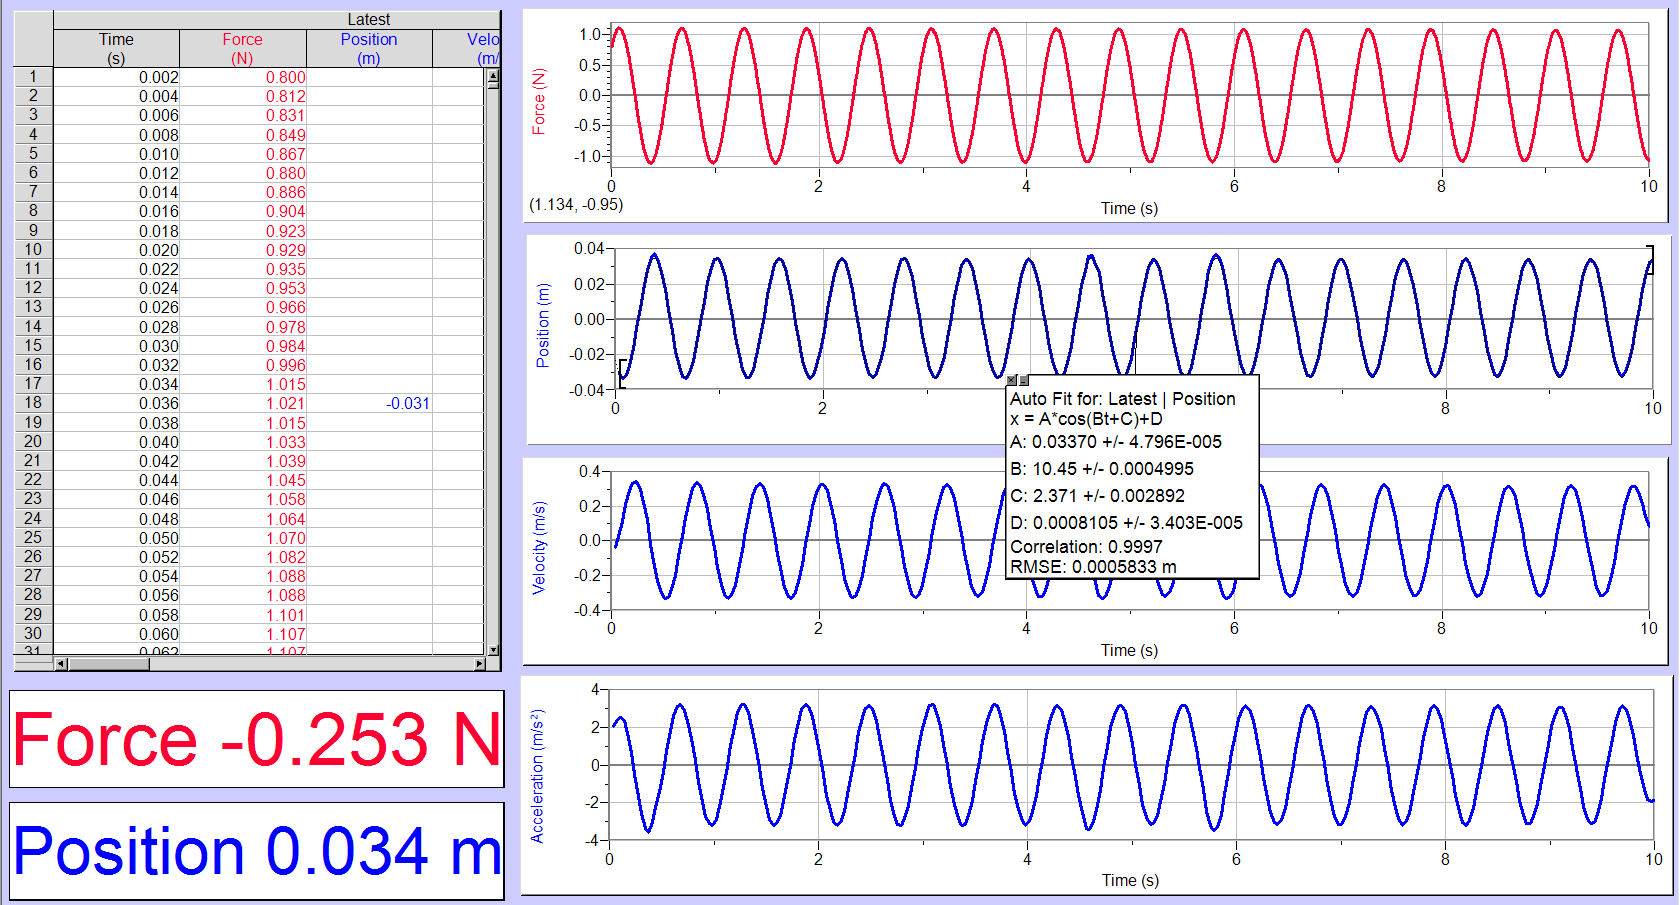
\includegraphics[width=\textwidth]{res/2_1_spring}
	\caption{Oscillations of Both Springs}
	\label{fig:Oscillations of Both Springs}
\end{figure}

\begin{figure}[H]
	\centering
	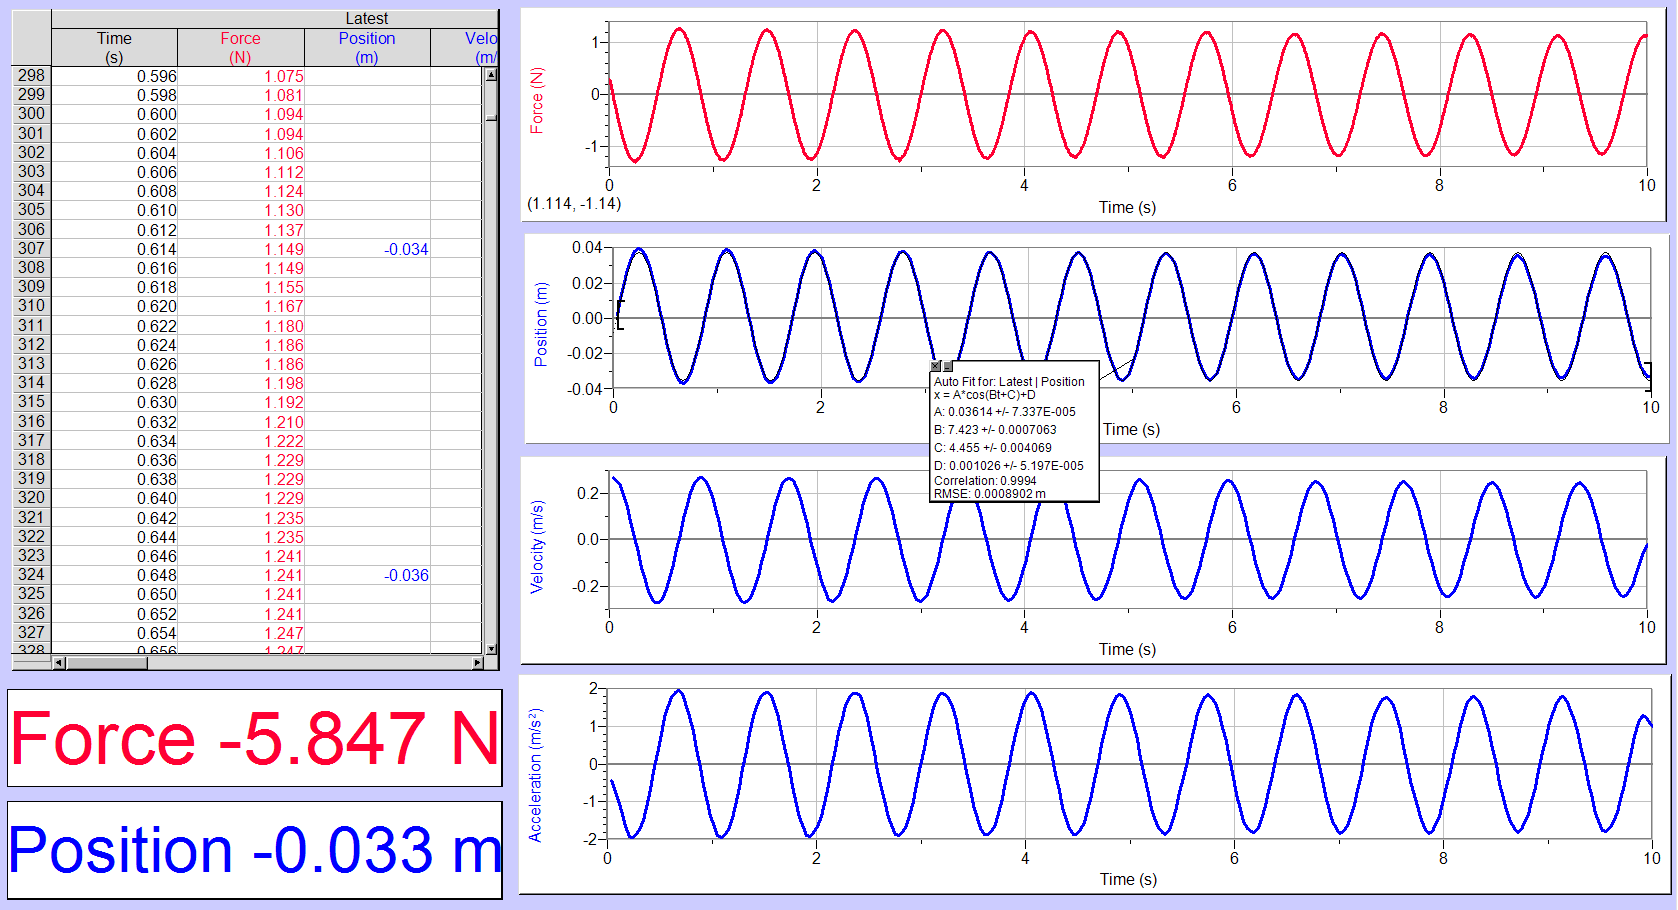
\includegraphics[width=\textwidth]{res/2_4_spring}
	\caption{Oscillations of Both Springs}
	\label{fig:Oscillations of Both Springs}
\end{figure}


\section{Discussion}
The theory predicted that the \textit{k} value of four springs springs in both series and parallel would be described by Equation \ref{parallelInSeries} (reproduced here for clarity):

\begin{equation*}
k_{seriesParallel}=\frac{1}{\frac{1}{k_1+k_2} + \frac{1}{k_3+k_4}} = k \tag{\ref{parallelInSeries}}
\end{equation*}

The position, velocity, and acceleration graphs had a nice structure to them. The velocity graph was phase shifted by $ \frac{\pi}{2} $ radians - the exact amount we would have expected from the equations. Furthermore, the acceleration graph was once again shifted $\frac{\pi}{2} $ radians from the velocity graph, and it followed the exact opposite of the position graph. This behavior follows nicely from the equations in the Introduction and Background section.

The phase shifting occurs for an intuitive reason. Force and acceleration peak at the same time. The velocity is zero when the acceleration is at its maximum, because the spring is stretched all the way and the mass is reversing direction. Finally, the distance is zero when the velocity is at its maximum because the mass is crossing its equilibrium point.

Putting the springs in series did, in fact, change their k values according to equation \ref{seriesSpring}.

\end{document}          
